\part{Visualiser les  simulations}

\chapter{Introduction à la visualisation de données}
\label{sec:visu}

Nous avons abordé en guise d'introduction un principe de base de la méthode scientifique: le cycle \textit{Observation -> Théorie -> Expérience}.
La visualisation représente l'étape de bouclage de ce cycle  puisque qu'elle consiste à observer le résultat de l'expérience de simulation.
Elle est importante car elle permet d'obtenir énormément d'informations facilement et rapidement.
Le cerveaux humain est efficace pour identifier les motifs qui se détache visuellement de leur environnement.
Elle permet une première approche qualitative qui va ensuite permettre de cibler une seconde approche plus quantitative.

%Par exemple, on peux utiliser une visualisation de la distribution de gaz autour de certaine galaxie pour identifier leur environnement, et ensuite l'étudier un fonction de la masse du halo hôte.
%La visualisation représente la première étape dans l'observation de la simulation.
%leurs forme, pour ensuite chercher a quantifier leurs forme en fonction de leurs halo hote.
%On peut facilement observer a l'oeil les motifs en forme de papillon des bulles d'ionisation.
%Ou la structure en réseau de la matière a grande échelle.
%La visualisation de donnée scientifique 


%pour qui?
En fonction du publique auquel s'adresse la visualisation, l'information utile sera différente et l'accent sera mis sur différents aspect.
%Il existe tout un panel de visualisations possible, et avant même de définir un but il faut définir une cible, car les outils ne seront pas les mêmes en fonction de la cible a laquelle ils s'adressent.
On distinguera principalement trois catégories de public:

\begin{itemize}
\item Le grand public. 
 
Il sera principalement touché par les images de vulgarisations que l'on peut trouver sur internet ou dans les magasine.
Ce type d'image n'a pour seul but que d'être artistique et agréable a regarder.

\item L'éducation.

Les images a vocation éducatives se doivent aussi d'être belles, mais elles doivent également comporter une partie informatives.
Elle doivent contenir une certaine dose d'information supplémentaire par rapport aux images purement artistique.

\item Les professionnels.

Enfin, les outils de visualisation pour les professionnels disposent généralement de tous les outils nécessaire à la quantification de l'information.
On pourra par exemple analyser différents champs physique, sous différents angles, changer les échelles de couleurs, etc.

\end{itemize}


% L'éducation 
%Ratio équitable entre qualification et quantification

%/ La vulgarisation
%Qualification principalement 
%il est important de créer des belles image

%Aligner des 1 et des 0 sur des gros ordinateur, n'a vraiment de sens que si il représente quelque chose.
%Le mot important dans cette phrase est représentation.
%Il est nécessaire, en recherche de visualiser ce qui se passe dans les simulations pour comprendre et qualifier les phénomènes avant de pouvoir les quantifier.
%Cette cible aura besoin d'outils pointu aillant pour principal objectif la quantification.

Le principal défi de la visualisation des simulations cosmologique est la quantité de données qu'elles représente.
Si il est possible de faire des rendu pré-calculés d'images, il est encore impossible d'avoir une représentation en temps réel de simulation de taille moyenne.
Pourtant il existe des techniques (dans le monde des jeux vidéo par exemple) permettant d'afficher dynamiquement des univers en 3 dimensions gigantesque de manière fluide sur des machines grand public.
Je pense qu'il y a de quoi s'inspirer de ce coté la.

Nous avons vu %TODO ref
qu'il existe deux types de représentation de la physique dans la simulation : la grille et les particules.
Ces deux représentation utilisent chacune des techniques de visualisation particulières.
Dans la suite de cette partie nous allons aborder séparément ces types de représentations et survoler les contraintes et les techniques associées a chacune.

Nous commencerons par aborder la visualisation de données sur grille, puis dans un second temps nous nous concentrerons sur la représentation des particules.
%Pourquoi

%Le monde de la 3D.
%Les simus, les moteurs de jeux video, les SFX de films,
%La 3D est partout.
%Les monde des simulation peux s'en inspirer.

\section{Projeter une grille AMR}

EMMA travail dans un espace en trois dimensions.
Nous cherchons ici à créer une image des résultats produit par EMMA.
En sortie d'EMMA, l'information est sous forme de liste de cellules \ac{AMR} disposant d'une position et d'une taille, dans un espace en trois dimensions.
Une image est composée d'une matrice à deux dimensions de pixels, généralement réguliers en forme et en taille.
Il est donc nécessaire d'effectuer une transformation entre ces deux représentations.
Cette transformation (on parlera de projection) mène a la perte d'une dimension, qui sera réduite a l'aide de lignes de visées.


\subsection{Le tirage des lignes de visées}

%La représentation d'un environnement virtuel a 3 dimensions passe toujours par la création d'une image a deux dimensions.
Il existe différents types de méthodes de projections qui dépendent de la gestion des lignes de visées.
Dans la suite de ce chapitre nous allons développer deux d'entre elles: la projection en perspective et la projection orthogonale (Fig \ref{fig:raycast_projection}).

\paragraph{La projection orthogonale} correspond a l'approximation de grande distance.
Les rayons sont parallèles entre eux et le cube de données est comme "écrasé" ou "imprimé" suivant un axe donné.
Cette projection est moins naturelle, dans le sens où elle ne correspond pas a ce que nous avons l'habitude de percevoir, mais elle a l'avantage d'être relativement simple a mettre en œuvre.

\paragraph{La projection en perspective} correspond au cas l'observateur est ponctuel et au centre d'une sphere, les rayons lumineux lui arrive radialement.
C'est la projection qui se rapproche le plus de la vision "naturelle".

\begin{figure}[bth]
    \center
    \subfloat[Orthogonale]{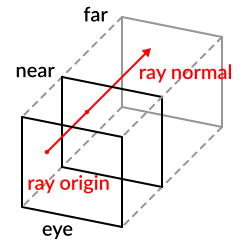
\includegraphics[width=0.45\textwidth]{img/04/raycast_ortho.png}}%
    \qquad
   	\subfloat[Perspective]{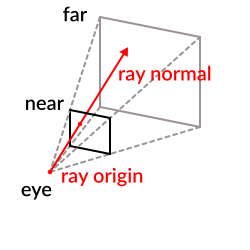
\includegraphics[width=0.45\textwidth]{img/04/raycast_perspective.png}}%
    \caption{Les deux types de projections que nous allons aborder.}
 	\label{fig:raycast_projection}
\end{figure}


\subsection{La réduction des lignes de visées}

Avant d'aborder le tirage des lignes de visées a proprement parlé, voyons rapidement comment les réduire une valeur unique pour effectuer la projection.
Il existe différentes façons de réduire les lignes de visées, en voici quelques une que j'ai pu utiliser:

\begin{itemize}
\item La moyenne ou la somme ont l'avantage d'être facilement implémentable et de garder l'information sur toute la ligne de visée.

\item Le maximum permet d'augmenter significativement le contraste, rendant les images visuellement plus intéressante que la moyenne/somme mais en contre partie certaines projections peuvent présenter des artefacts indésirables.

\item L'épaisseur optique permet de garder de l'information sur toute la ligne et d'être une représentation avec une signification physique car elle utilise les équations de transfert du rayonnement.
Cependant elle est plus gourmande en ressources.
Pour faire de la visualisation pure on pourra utiliser une expression du type:
\begin{equation}
v= \sum e^{-x}
\label{eq:epop}
\end{equation}
Et on pourra également être plus quantitatif en utilisant les vraies équations physique mais il faudra utiliser plusieurs champs simultanément. %TODO ref

\item D'une manière générale, toute transformation permettant d'obtenir une seul valeur a partir d'une série

\end{itemize}

%Une des méthodes les plus facile consiste a prendre la moyenne ou la somme de la ligne, cette méthode présente l'avantage de représenter l'ensemble de la ligne.
%Il est également possible de prendre les maximum de la ligne, cette méthode augmente significativement le contraste, au point que certaines projections peuvent présenter des artefacts indésirables.

%Une troisième méthodes légèrement plus physique consiste a utiliser les équations de transfert du rayonnment pour determiner l'epaisseur optique de la ligne

%Enfin, il est possible d'utilisé la réelle expression de l'epaisseur optique, prenant en compte densité, température, ionization et vitesse du gaz.
%(TODO)

\section{Projection orthogonale}

La projection orthogonale est la plus directe car tout les rayons sont parallèles entre eux et suivent un axe de la grille.
Comme la grille est ici composée de cellule de différentes taille, il faut prendre en compte l'étendue spatiale de chaque cellule de manière individuelles.

J'ai développé une méthode de projection d'\ac{AMR} sur une grille (2D ou 3D) de taille arbitraire en utilisant des histogrammes.
Ces fonctions étant très bien optimisées, la performance de génération des cartes/cubes est généralement satisfaisante (de l'ordre de quelque secondes pour un cube de $1024^3$ avec les fonctions histogramme de Numpy).
L'idée est de considérer les cellules \ac{AMR} comme des particules et de les projeter niveau par niveau.


%Prenons l'exemple de la densité sur une grille non raffinée utilisant le format de sortie d'EMMA.
%Une grille 2D quelconque est représenté par le couple $x,y$ étant les positions du bord inférieur gauche des cellules, $l$ étant le niveau des cellules et $d$ étant le champs a représenter (prenons par exemple la densité).

Par exemple, prenons comme objectif de projeter la densité de gaz provenant d'une grille \ac{AMR} 3D de niveau de base $L_{0}=8$ sur une matrice 2D $256^2$.
En réalisant un histogram 2D, sur les positions $x$ et $y$ des cellules, on obtient directement un projection suivant l'axe $z$ de la grille \ac{AMR}.
Les valeurs de toutes les cellules aillant des positions comprise dans un intervalle (x+dx,y+dy) seront automatiquement ajoutées au pixel correspondant.

Cependant, dans le cas d'une grille raffinée, il est nécessaire de prendre en compte une pondération pour les cellules raffinées.
Le volume d'une cellule est définis en fonction de son niveau $dV= 2^{-3L}$, et son poids $w$ en fonction de la valeur $\rho$ à projeter sera $w = \rho \cdot dV$.
L'image finale sera alors obtenue en réalisant un histogramme 2D pondéré par $w$.

%En réalisant un histogram 2d de x et y pondéré en masse.

%En considérant le centre des cellule $(x' = x+dx(L) /2)$ et en ajustant le bin de l’histogramme sur la taille de la grille on peux projeter un niveau rapidement.

%\begin{lstlisting}[float=bth,language=python,frame=tb,caption={lprojection de l'AMR par la méthode des histogramme Numpy},label=lst:useless]
% import numpy as np
% h,binX,binY=np.hystogram2d(x,y,weight=dv)
%\end{lstlisting}
%u h est une matrice 2d representant la projection.
%Lorsque l'AMR d'entrée contient plusieurs niveaux, il est possible de projeter les cellules niveau par niveau.


Ceci n'est valable que dans le cas d'une projection sur le niveau de base de la grille \ac{AMR}.
Cependant il est possible de projeter la grille a une résolution supérieure.
Prenons par example pour une grille contenant de niveau $L_{0}=8$ raffinée une fois.
Pour obtenir une image $512^2$, on projettera d'abord toutes les cellules de niveau 8 (et seulement ces cellules) pour obtenir une matrice $256x256$.
On agrandira cette matrice avec des opérateurs de changement de grille (cf Section \ref{Opérateurs de changement de grilles}).
%La méthode la plus naturelle consiste utiliser une projection directe.
Nous obtenons alors une première grille de taille $512x512$ présentant des trous aux emplacements des endroits raffinés.
On projettera ensuite de la même manière les cellules du niveau $L=9$ pour obtenir une seconde matrice de taille $512x512$.
Cette seconde matrice sera finalement utilisée pour combler les trous de la première.
%En prenant la moyenne des deux grille obtenues ont obtient finalement la projection sur le niveau $L=9$.
%On pourra utiliser ce principe de manière récursive jusqu'à avoir projeter tout les niveaux.

Dans le cas ou le niveau de projection ne correspond pas au niveau maximum de l'\ac{AMR}, il suffira de modifier la pondération des niveau supérieurs au niveau de projection en utilisant:
\begin{equation}
w = d \cdot \left( 2^{Lmax-L} \right)^3
\end{equation}
Ainsi toute les cellules se trouvant sur des niveaux supérieur au niveaux de projection seront automatiquement prisent en compte.

Le principal inconvenant de la méthode des histogrammes est qu'il n'est possible de réaliser que des projection utilisant la moyenne.
Or on voudra dans certain cas considérer d'autres réduction de ligne de visée.
Dans le cas de la création d'une carte 2D de maximum par exemple, il est nécessaire de générer un cube avant de réaliser la projection.
L'avantage est que cette méthode est aisément transposable a trois dimensions en utilisant des histogrammes 3D.


%Pour compenser ce problème on réalisera une projection 3D de la même manière que précédemment mais en utilisant de histogrammes a 3 dimensions.
%Il sera ainsi possible de réduire le cube obtenu de  
%La taille de l'histogramme augmentant en $2^{3L}$ les projections 3D seront généralement limité a $1024^3$ pour des questions de mémoire RAM. 


J'ai utilisée cette méthode pour projeter quelques champs de données de la simulation CODAII-EMMA.
Un exemple d'image réalisée est présenté sur la figure \ref{fig:ortho}.
Pour réaliser cette image j'ai projeté une tranche de 8/h cMpc d'épaisseur sur le niveau de base.
Cette projection a été effectuée trois fois, pour la température, la densité et l'état d'ionisation du gaz.
L'image finale est une composition \ac{RGB} de ces trois champs.

J'ai également généré des images de $16384^2$ pixels (256 Megapixel), en découpant le cube en tranche sur lesquelles j'ai effectué une projection par moyenne.
J'ai ensuite réalisé un maximum sur les tranches obtenues pour générer l'image finale.

%La quantité de données a gérée étant importante,

%Pour afficher l'image en ligne de manière fluide j'ai utilisé Openseadragon %TODO ref
%un logiciel permettant d générer des tuiles d'images et de les charger dynamiquement.
%Ces images sont disponibles en lignes a l'adresse %TODO ref

\begin{figure}[bth]
        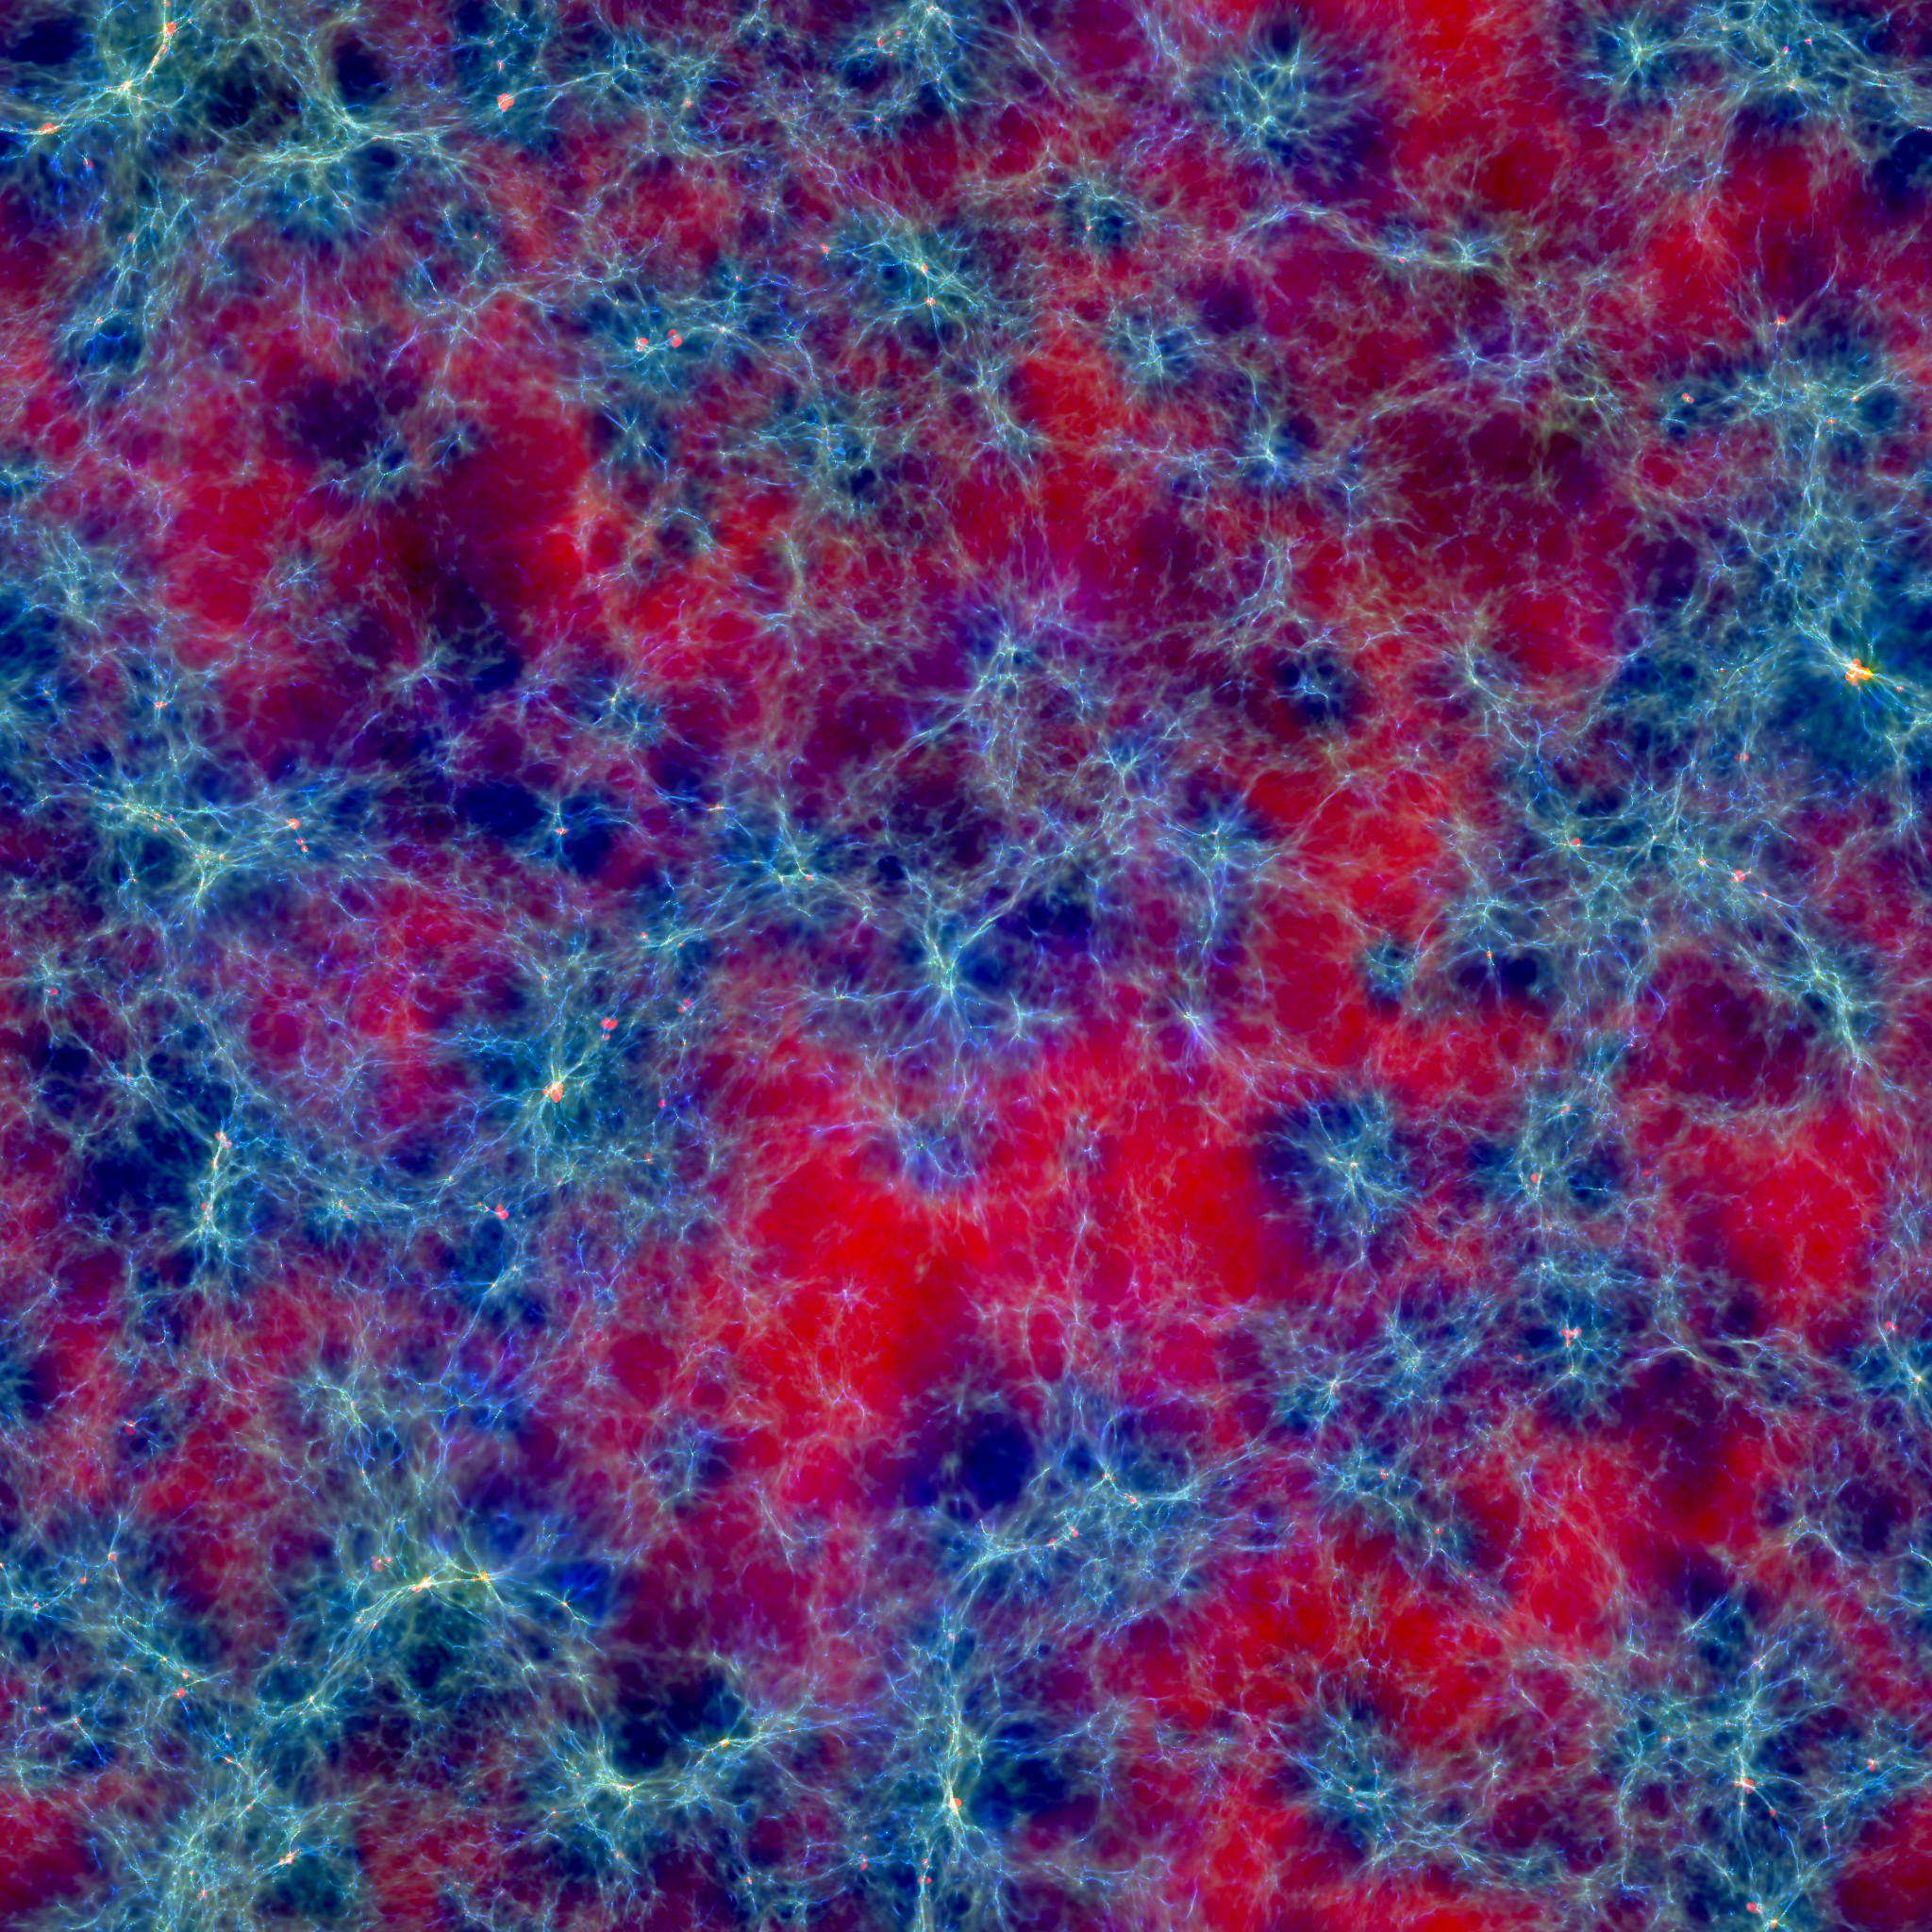
\includegraphics[width=.95\textwidth]{img/04/rgb-compose.jpeg} 
        \caption{Projection orthogonale de la simulation CODAII- EMMA sur une matrice $2048^2$.
        La projection correspond à la moyenne sur une tranche de 8/h Mpc d'épaisseur. 
        La composition RGB est réalisée avec dans l'ordre la température, la densité de gaz et la densité de gaz ionisé.
		Les vaste zones rouges correspondent aux vides qui ont reçut du rayonnement plus tard et n'ont pas encore eu le temps de refroidir par détente adiabatique.  
        }
 		\label{fig:ortho}
\end{figure}


\clearpage
\section{Projection en perspective}
%opengl
%blender

Dans le cas de la projection en perspective, les lignes de visées ne sont plus parralèles, et il n'existe plus de façon directe de les récupérer.
Il devient nécessaire d'avoir recours au lancé de rayon.
Cette technique, appelée raycasting, permet de récupérer toute les cellules interceptée pas un segment de droite donné.
%Il existe différentes techniques de raycasting, j'ai pu en explorer plusieurs:

\subsection{Raycasting}
\subsubsection{L'algorithme de bressenham}
L'algorithme de Bressenham est une technique optimisée de raycasting.
Il consiste a manipuler des indice de cellules pour déterminer quelles cellules intercepte un segment arbitraire.
Cette technique est rapide mais ne fonctionne cependant que sur grille régulière.
Il est donc nécessaire de projeter la grille à la résolution désirée avant de tirer les rayons.

\begin{figure}[bth]
        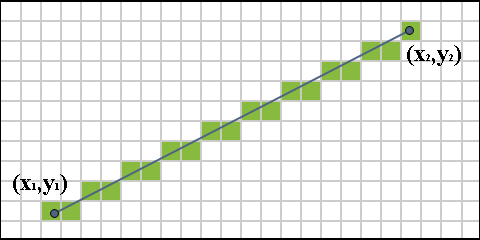
\includegraphics[width=.95\linewidth]{img/04/Bresenham_line.png} 
        \caption{Algorithme de Bressenham }
 		\label{fig:bressenham}
\end{figure}

\subsubsection{La méthodes KD-tree}

J'ai mis en place une autre technique dans le but d'explorer directement l'\ac{AMR} et éviter la projection sur grille régulière.
De la même manière que la technique de calcul des flux (voir partie \ref{sec:healpix}) cette technique repose sur l'utilisation d'un arbre pour déterminer les cellules par lesquelles passent le rayon.
La première étape consiste à tracer une ligne de vidée dans l'espace et de la discrétiser.
Pour chaque vertex de cette ligne on utilisera le KD-tree pour déterminer qu'elle cellule \ac{AMR} est la plus proche de ce vertex.
Enfin on associera la valeur de cette cellule au vertex en question.
Cette technique nécessite la génération de l'arbre sur la grille mais a l'avantage d'économiser le temps de projection de l'\ac{AMR} sur une grille régulière.


\subsection{Application}

%la mise en place de la camera
%la définition de la position et du champs de vue (FOV) et de la profondeur de vue.

\begin{figure}[bth]
        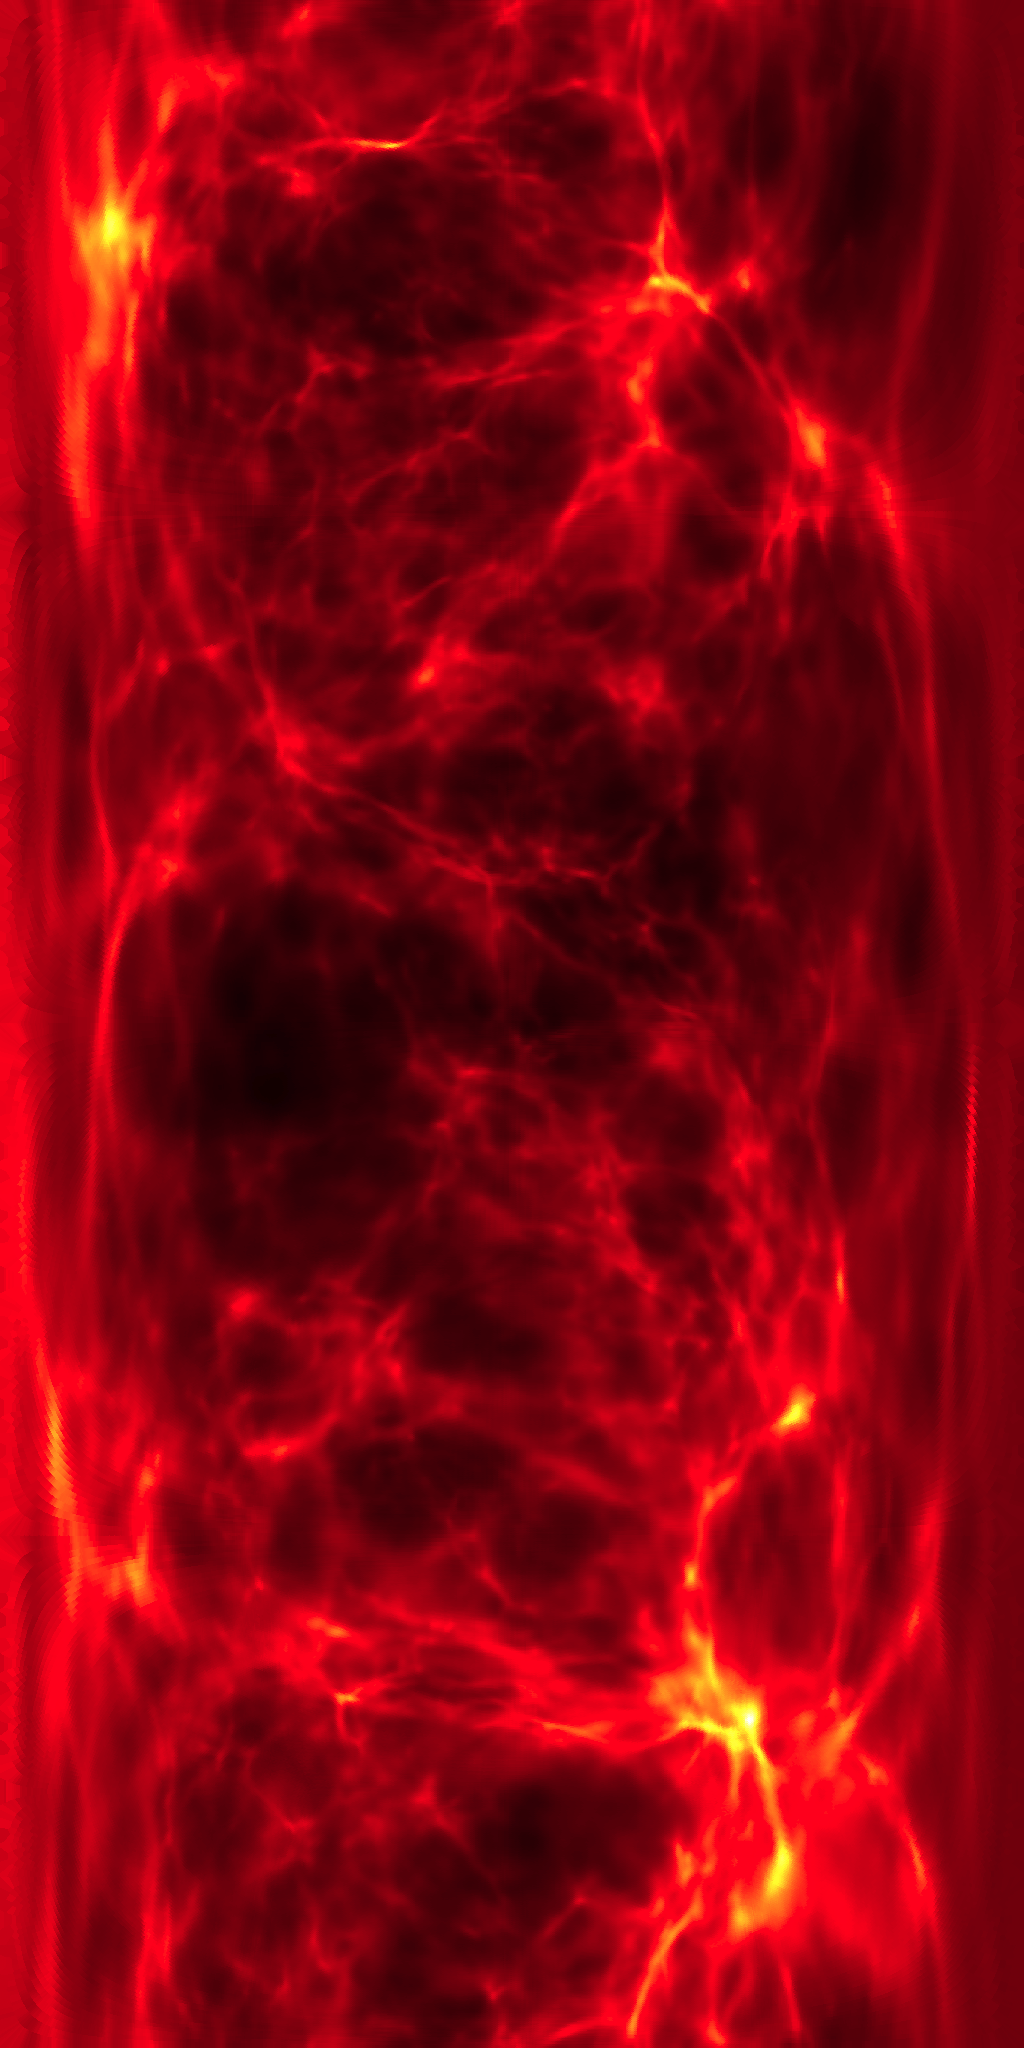
\includegraphics[height=.95\textheight]{img/04/equi.png} 
        \caption{Projection equirectangle d'une cube de densité.
        Ce type d'image représente une vue de $360°$ par $180°$ (d'ou un ratio d'aspect de $2:1$) ici prise depuis le centre de la simulation.}
 		\label{fig:equirectangle}
\end{figure}

Indépendamment de la méthode de lancé de rayon, il est nécessaire de définir la caméra.
C'est a dire qu'il faut localiser le point de départ (la position de la caméra) et les points d'arrivés (\ac{FOV} et profondeur de champs) des rayons.
Pour l'exemple présenté sur la figure \ref{fig:equirectangle}, la caméra est positionnée au centre d'un cube de densité de gaz $P_i = (0.5,0.5,0.5)$.
J'ai ensuite défini une caméra sphérique avec HealPix (see Sec. \ref{sec:healpix}) pour lancer les rayons dans la sphère inscrite au cube.
La projection a utilisée ici $786432$ rayons et chaque rayon à utilisé la réduction de l'équation \ref{eq:epop}.

Il est ensuite nécessaire de projeter la sphère sur une surface plane.
J'ai utilisé la projection equirectangle qui est la projection la plus utilisée en photographie et vidéo sphérique.
Elle présente un ratio d'aspect de 2:1 correspondant a un \ac{FOV} de 360x180°.

%L'association Healpix vers equirectangle est trivial puisque qu'elle consiste a associer les position x,y de la projection equirectangle, au angle $\theta$ et $\phi$ de la projection Healpix.
Cette projection est triviale puisqu'elle consiste à associer les positions cartésiennes des pixels aux angles des rayons:
\begin{equation}
x=\theta\\
y=\phi.
\end{equation}

La densité de point n’étant pas uniforme dans ce référentiel, il est nécessaire de réaliser une interpolation sur une matrice régulière pour obtenir l'image finale.
Ce type d'image se prêtent bien a la vulgarisation, car le résultat final est léger et peut être utilisé avec un visualisateur de type Google Cardboard par exemple pour obtenir une visualisation interactive facile à diffuser.

Il est également possible d'utiliser ce type de méthode à des fin plus quantitatives.
En fonction de la méthode de réduction des rayons, il peut être possible d'étudier, pour des halos spécifiques, la fraction d'échappement des photons ou les flux hydrodynamiques en fonction de la direction. 
Il est également possible de créer des observatoires virtuels en simulant différents types d'instruments.

%\section{le compositing RGB (A)}
%Une fois les projections réalisées il est possibles de les combiner en créant des images en fausses couleurs.
%
%De manière naturelle, J'ai utilisé le rouge pour la température et la transparence pour l'ionisation.
%il reste le bleu et le vert.
%Dans une première série d'images j'ai utilisé le vert pour la densité de gas et le bleu pour la densité de matière noire.
%
%\subsection{le théorie des couleurs}
%Comment créer du noir et blanc?
%
%
%par la moyenne :
%\begin{equation}
%gray= (R+G+B)/3
%\end{equation}
%
%R,G,B=gray
%
%
%par une ponderation spéciale correspondant a la capacité de l'oeil a voir certaine couleur, conservation de la luminance:
%\begin{equation}
%gray = R*0.2989 + G*0.5870 +B*0.1140
%\end{equation}
%
%R,G,B=gray




\section{Movie}
%implementation du mode movie de EMMA
%c'est la même chose que précedemment mais a chaque pas de temps, il faut l'implementer en live (en c) pour ne pas avoir a sortir toute les info.


J'ai implémenté dans EMMA, la possibilité d'obtenir une matrice 2D par pas de temps, représentant la projection orthogonale suivant un axe donné.
La projection est réalisée de la même manière que précédemment mais a la volée et à chaque pas de temps.
Le choix a été fait de réaliser la projection a la fin de chaque pas de temps du niveau de base, ce qui limite la résolution temporelle a celle du niveau de base.

%Comme la résolution temporelle des niveaux raffinés est plus importante que le niveau coarse, la projection temporelle peux etre 
%En écrivant ces lignes je me rends compte que le dt de projection devrait être lié au dx de projection. 

Les simulations que j'ai pu réalisées comportaient environs un millier de pas temps, et généraient donc autant d'images ($N_{dt} \approx 10^3$).
A 25 \ac{FPS} cela représente une durée d'environs 40 secondes de vidéo.

\section{Light cone}

A partir des images générées par le mode movie, il est possible de créer une image composite appelée "light cone".
Un "light cone" est une image aillant une dimension spatiale sur un axe, et une dimension temporelle sur un second axe.

En effet, il est possible de voir un film comme étant un parallélépipède avec deux dimensions spatiales et un dimension temporelle.
En projetant ce parallélépipède sur un axe spatial, on obtient un "light cone"
On parle de cone car en unités physique, la taille de la simulation augmente avec le temps, et donc, le parallélépipède s'élargit, formant un cone.

%La création d'un "light cone" se fait a partir des images générer par le mode movie.
En pratique, l'idée est de prendre des fines tranches successives dans les sorties movie.
Si les images en sorties du mode movie ont une résolution $N_p=1024$ pixel carré.
On prend une tranche d'une épaisseur $dx$ donnée suivant l'axe $y$ sur l'image du pas de temps $i_{dt}$, puis une deuxième tranche de la même épaisseur, mais décalée de $dx$ dans l 'image $i_{dt+1}$, et ainsi de suite.
La position du début $S_i$ et de la fin $S_f$ de la tranche dans l'image sera :

\begin{equation}
S_i = (dx \cdot i_{dt}) \% N_p \\
S_f = S_i + dx 
\end{equation} 

Le modulo sur la taille de l'image permet de gérer les conditions périodiques simplement.
On prendra également garde a utiliser une épaisseur de tranche qui soit un multiple entier du nombre de pixel de l'image de manière a respecter simplement les conditions périodique
Le ratio d'aspect $\Phi$ est le rapport entre la hauteur et la longueur de l'image, et s'exprime :
\begin{equation}
\Phi = \frac{ N_{dt} * dx}{N_p}
\end{equation}
Étant donné que $N_{dt}$ et $N_p$ sont fixés par les paramètres de la simulation, il n'est possible de gérer le ratio d'aspect qu'en fonction de l'épaisseur de la tranche $dx$.
Plus le ratio d'aspect sera important, plus les structure vont se répéter sur le light cone.

Un light cone réalisé avec cette méthode et à partir d'une simulation présentée dans la partie \ref{sec:etoiles} est présenté sur la figure \ref{fig:lightcone}
L'image résultante est un composite \ac{RGB} de la densité de matière noire, de la densité de gaz, de la température et de l'état d'ionisation.

\begin{figure}[bth]
        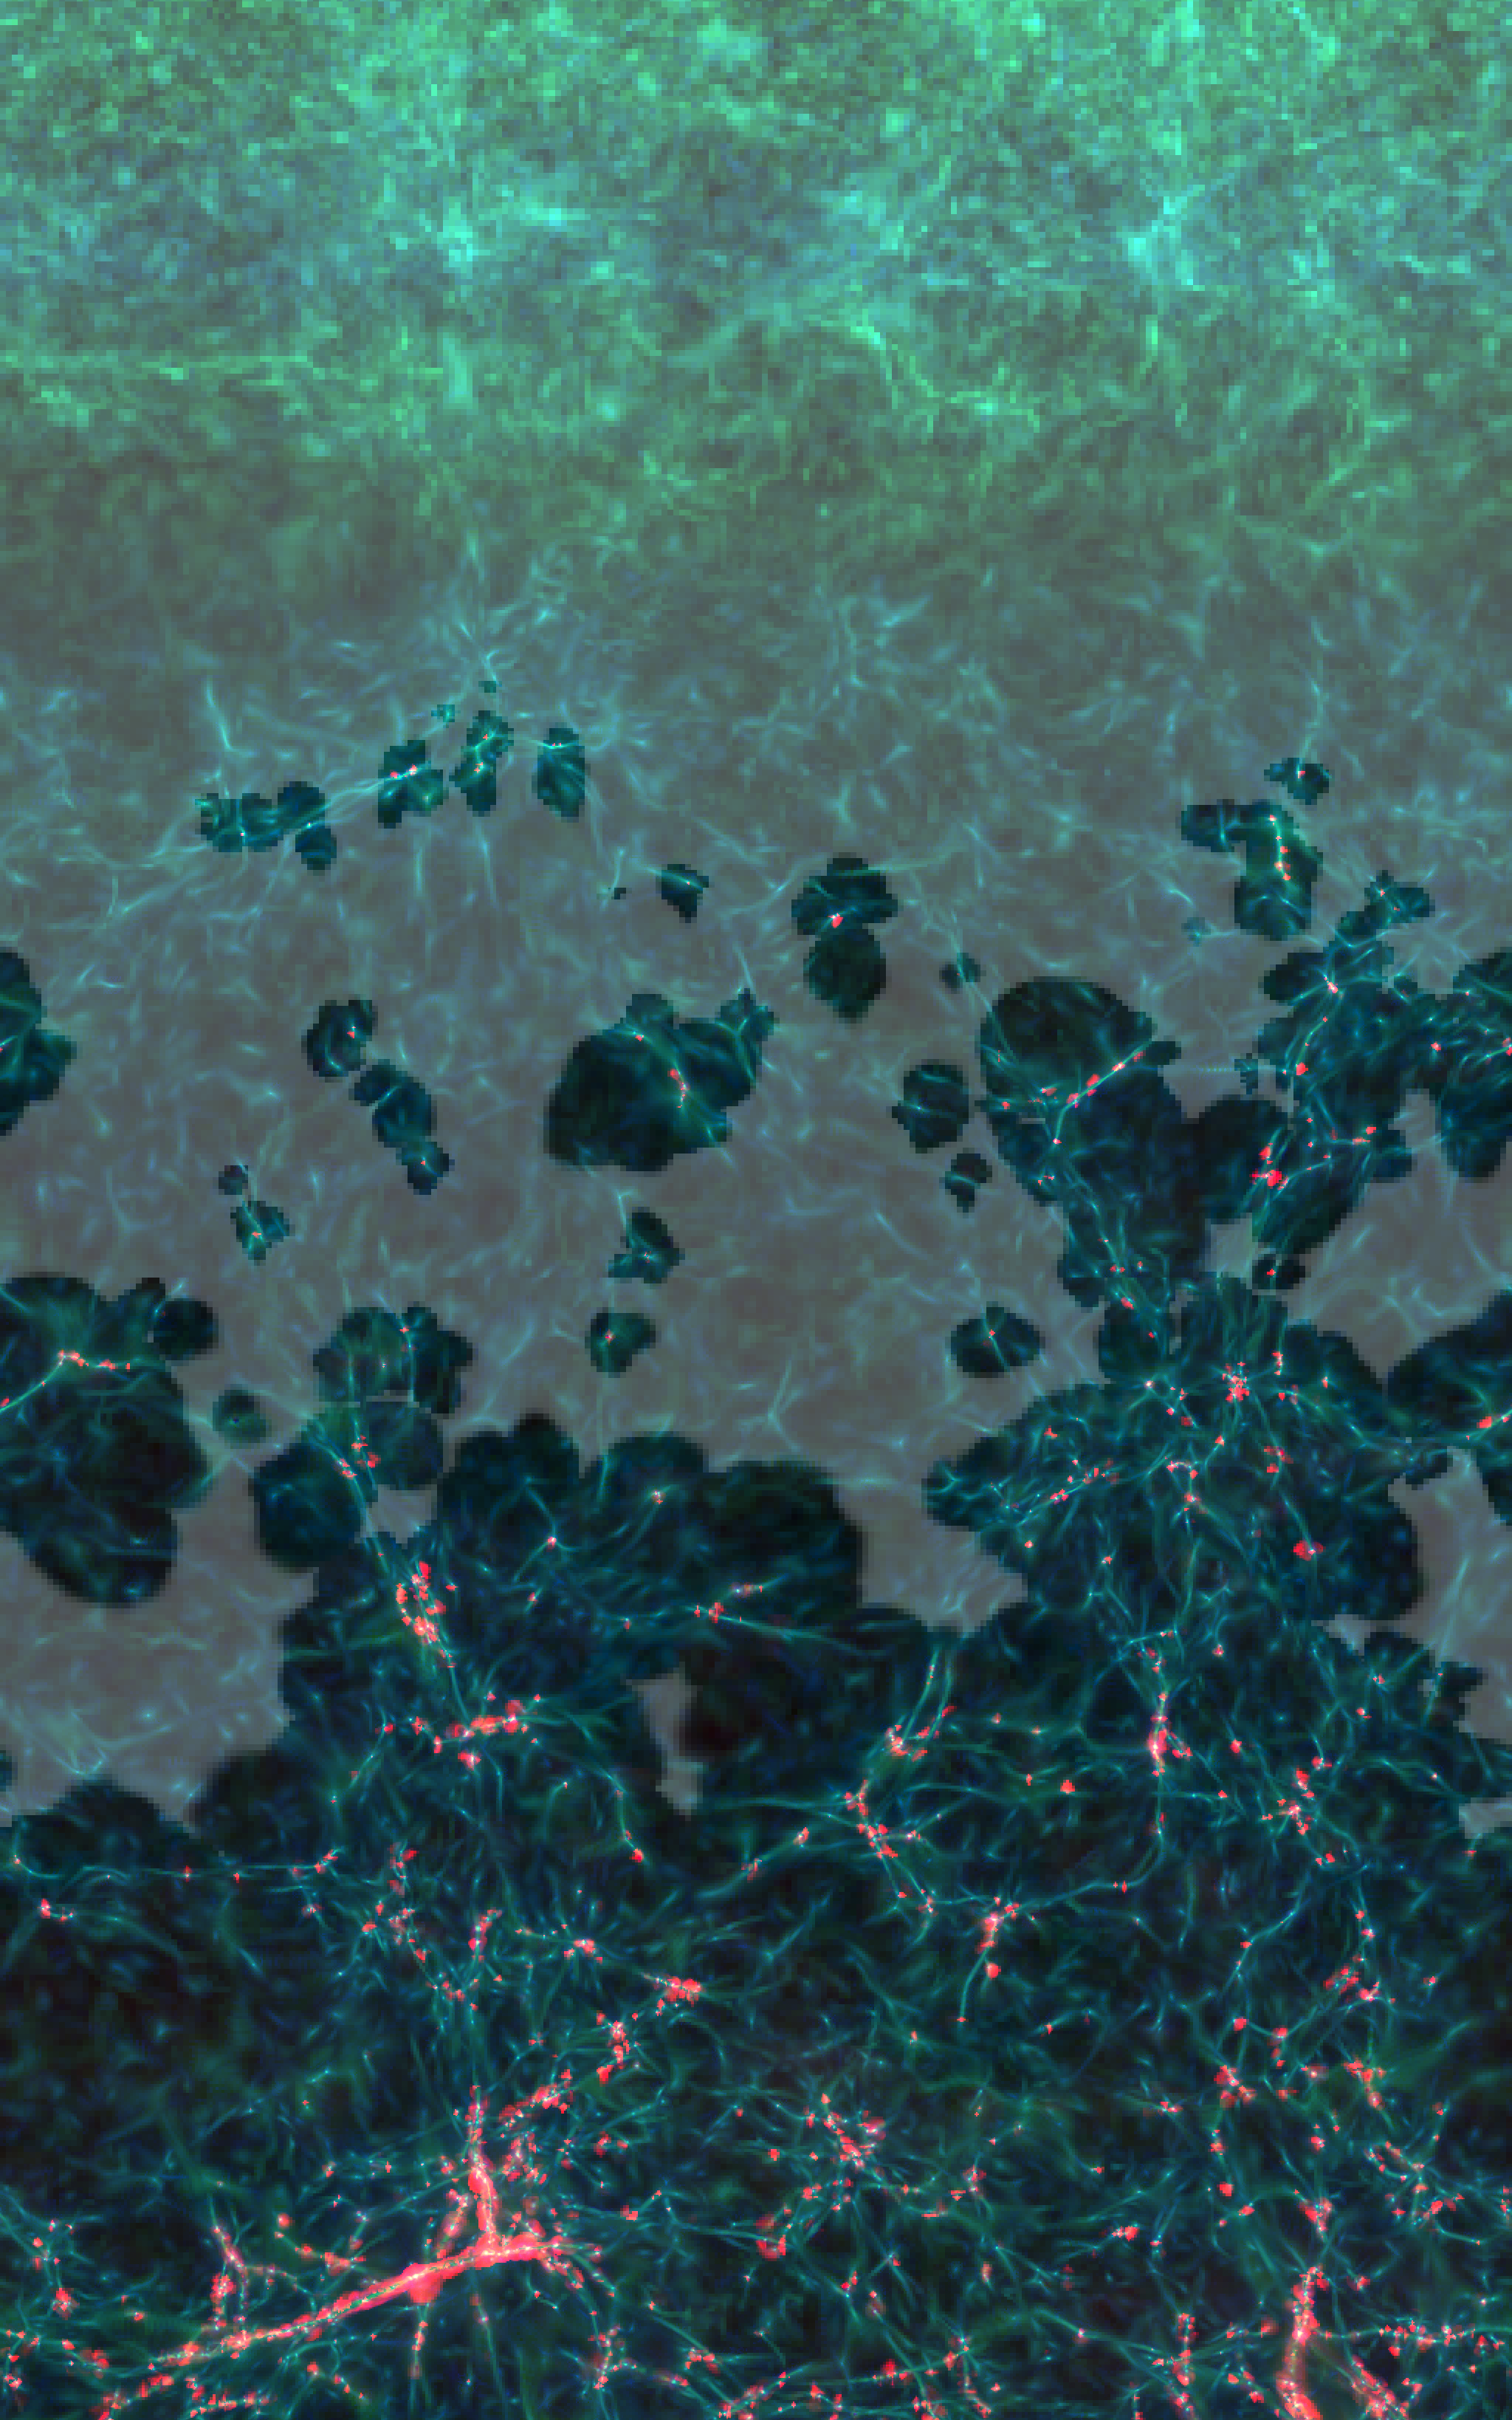
\includegraphics[height=.90\textheight]{img/04/frise_wall.png} 
        \caption{Light cone dans une simulation $8/h Mpc ^3$. 
        Le temps se déroule de haut en bas sur plus de 700 Myrs.
        Le voile blanc représente l'état d'ionisation du gaz.
        L'apparition des bulles d'ionisation est clairement localisée autour des structures les plus denses.
        Le rouge représente les température de plus de $2\cdot 10^4K$ pour accentuer les supernovae. 
 }
 		\label{fig:lightcone}
\end{figure}

\section{Projection interactive en 3D}
%\subsection{avec un frame work} 
%
%Blender 
%interface python
%Logiciel de visualisation 3d
%Possibilité de faire du rendu volumique de qualité professionnelle
%Pas adapté a la visu scientifique.
%
%
%Irlicht
%Moteur de jeu 3d open source 
%extremement simple d'utilisation
%les particules sont des bilboard : de texture 2d qui pointent tjrs vers la caméra
%posibilité de customiser les points
%deplacement en temps réel dans l'univers 3D a la manière d'un FPS
%(tres) mauvaise performance 
%\subsection{Sans Framework}


Les projections présentées jusqu'ici sont toutes des projections pré-calculées de grille \ac{AMR}.
Dans cette section nous nous concentrons sur la visualisation de données sous formes de particules, et avec l'objectif de pouvoir explorer ces données en temps réel. 
Explorer les simulations produites en trois dimensions et en temps réel, permettrait un énorme gain de temps au niveau de l'analyse, puisqu'il serait alors possible de localiser visuellement et très rapidement les régions d’intérêts.

J'ai fait quelques essais de visualisations en temps réel en utilisant des frameworks existant.
%J'ai testé par exemple Blender %TODO ref
%un logiciel libre disposant d'une interface python qui permet de faire du rendu 3D professionnel et qui possède un moteur de jeux permettant de faire du temps réel.
J'ai par exemple utilisé \cite{Irrlicht} un moteur de jeu open source simple d'utilisation permettant des déplacements en temps réel dans un univers 3D à la manière d'un jeu de tir a la première personne.
L'utilisation de ce type de moteur de jeu permet l'utilisation d'une grande variété de fonction pré existante.
Ces fonction permettent de créer un monde, d'y placer des particules, de créer une camera et d'y associer des mouvements de façon intuitive.
De plus, Irrlicht possède un module Occulus Rift qui m'a permis d'explorer le monde ainsi créer en réalité virtuelle.
Ce test de visualiseur en réalité virtuelle a indirectement mené a la publication de l'article de conférence en annexe \ref{pap:visu}.

Son principal inconvénient est ses performances limitées.
Dans Irrlicht, l'affichage d'une particule se fait par l'intermédiaire d'un "billboard" qui est une surface rectangulaire faisant toujours face à la camera.
Une particule n'étant pas représentée par un simple point, le gain en performance peux être substantiel.
Dans le but d'obtenir de meilleur performance, j'ai développé un visualiseur de particule directement en OpenGL, un langage graphique bas niveau permettant de meilleurs optimisations que l'utilisation de moteurs de jeux préexistant.
Une capture d'écran d'un cube de $128^3$ particules de matière noire, rendu de ce viewer est présenté sur la figure \ref{fig:viewer}.
Ce nouveau visualiseur est capable d'afficher environs huit fois plus de particules que le précédent avant de ressentir des ralentissement notable a l'affichage. 

%LEs partivule sont des vertex en language OpenGL.
%declaration de buffer, envois sur la carte graphique.

En plus de la visualisation interactive, j'y ai ajouter la possibilité de déplacer les particules.
Pour cela, il faut interpoler les positions des particules entre deux instants.
La principale difficulté était de mettre a jour la position des particules.
OpenGL utilise un paradigme proche de CUDA.
Les positions des particules sont définies en mémoire sur le CPU puis envoyées sur le GPU pour l'affichage.
Lors des déplacements ces transfert était fait a chaque frame et ralentissaient considérablement les performances.
en utilisant une passerelle entre OpenGL et CUDA, j'ai pu réaliser les déplacement directement sur la carte graphique et économiser les temps de transferts.
Au final, la visualisation de la formation des structures de matières noires en temps réelle est très instructive.

Ce projet a néanmoins été mis de coté, car un projet bien plus ambitieux a été amorcé par A. Schaaff.
L'objectif est de réaliser un visualiseur capable de représenter un volume de donnée aussi conséquent que ceux de la simulation CODA.
Pour se faire, il utilise un système de base de données organisée en octree permettant un affichage adaptatif des particules en fonction de leurs distance.
Cet outil est réalisé en JavaScript et utilise les technologies web pour un affichage a distance dans un navigateur internet, les données en elle même étant stockées sur un serveur.
Les premiers pas de cet outil sont prometteurs, puisqu'il dispose déjà de modules de mesure et de sélection permettant un usage scientifique.


%Prochain objectif, ajouter du mouvement.
%Interpolation entre 2 snaps.
%interpolation faite en CUDA pour éviter les retour de GPU vers CPU.
%posibilité d'utiliser plusieurs snaps 
%Visualisation de la formation des structure en temps réélle tres instructive



\begin{figure}[bth]
        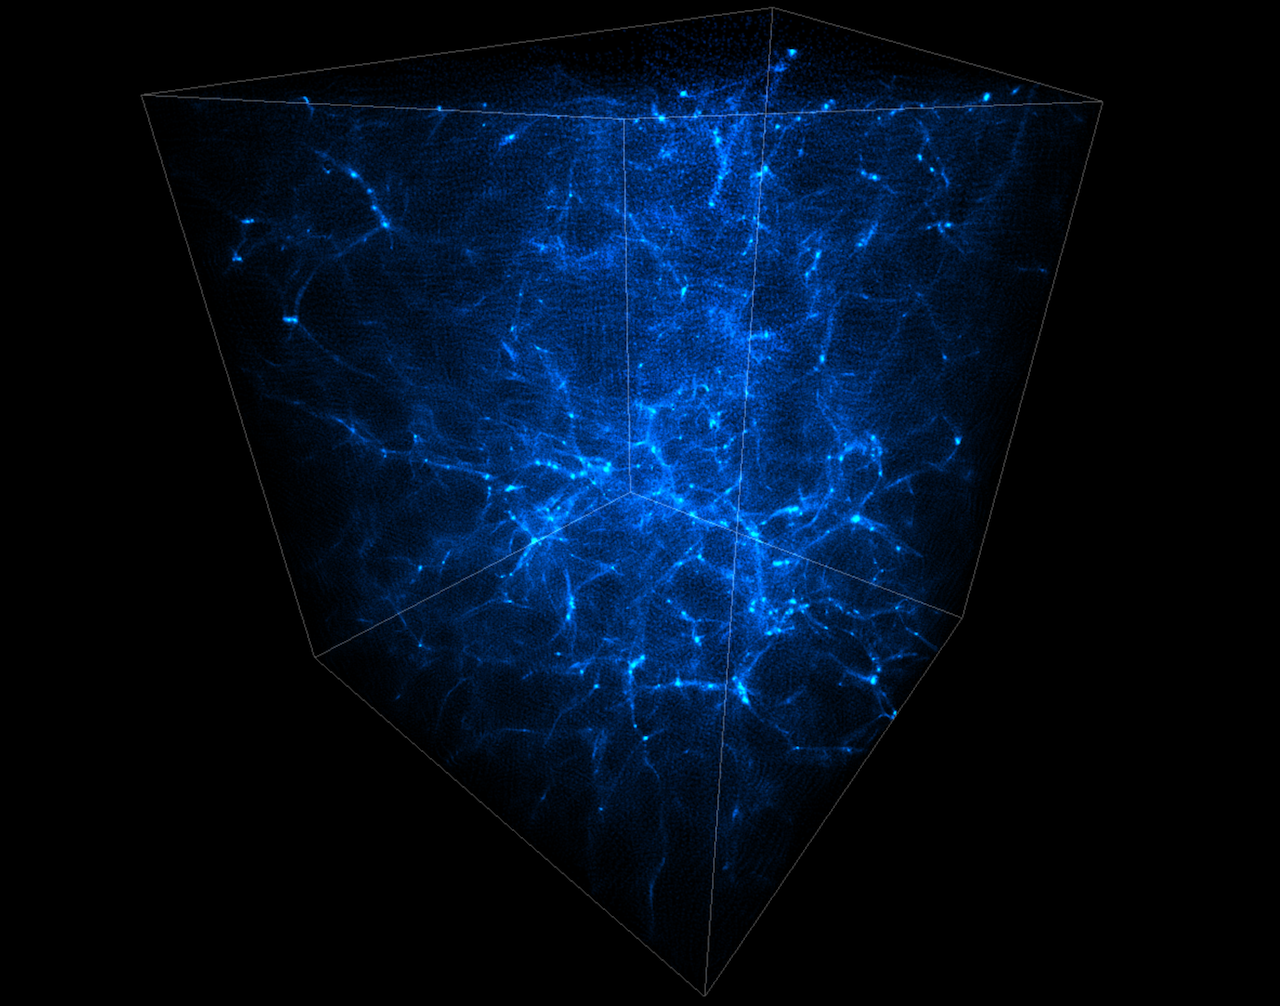
\includegraphics[width=.95\linewidth]{img/04/part.png} 
        \caption{Capture d’écran de mon viewer 3D en OpenGL.
        Le déplacement en temps réel dans un système de particules de matière noire en mouvement est très instructif.}
 		\label{fig:viewer}
\end{figure}


\section{Conclusion}

La visualisation de données de simulations cosmologique représente un véritable challenge et peux s'adresser a un large public.
Il existe différentes technique en fonction de l'objectif.
Les travaux présentés dans cette partie ne sont qu'un survol de ce qu'il est possible de faire.
Il existe des méthodes, déjà développées dans d'autres domaines qu'il serait intéressant d'exploiter à des fins de recherches.



